
\documentclass[10pt,a4paper,twoside,openright,fleqn,%
               parskip=half,%
               BCOR=5mm,DIV=10,footinclude=false%
               numbers=noenddot,cleardoublepage=empty]{scrbook}

\usepackage[utf8]{inputenc} 
\usepackage[sc]{mathpazo} %-- use Palatino font
\usepackage{amsmath,amssymb,amsthm}
\usepackage[square]{natbib}
\usepackage{subcaption} 
\usepackage{xspace}
\usepackage[breaklinks=true,
            colorlinks=true,
            linktocpage=true,
            allcolors=colorforlinks]{hyperref} 
\usepackage[ruled,vlined,algochapter,linesnumbered]{algorithm2e}
\usepackage{calc}
\usepackage{ccicons} 
\usepackage{xspace} 
\usepackage{booktabs} 
\usepackage[english]{babel}  
\usepackage{listings}
\usepackage{scrhack} % ignore warnings about deprecated KOMA-Script
\usepackage[printonlyused,smaller,withpage]{acronym}
\usepackage[usenames,dvipsnames]{xcolor}
\usepackage{graphicx}
\usepackage{pdfpages}
\usepackage{todonotes}






\newcommand{\myName}{Hidemichi Baba}
\newcommand{\myTitle}{FlatCityBuf: a new cloud-optimised CityJSON format}

\newcommand{\myGroup}{3D geoinformation group}
\def\myGroupLogo{figs/tud-3dgeoinfo-black.png}
\newcommand{\myUni}{Delft University of Technology}


\newcommand{\myGraduationYear}{2025}
\newcommand{\myGraduationMonth}{June}

\newcommand{\mySupervisorOne}{Asso.\prof.dr.\ Hugo Ledoux}
\newcommand{\mySupervisorTwo}{Dr.\ Ravi Peters}
\newcommand{\myCoreader}{Assi.\prof.dr.\ Martijn Meijers}


%-- for names for \autoref commands
\def\chapterautorefname{Chapter}
\def\sectionautorefname{Section}
\def\subsectionautorefname{Section}
\def\subsubsectionautorefname{Section}
\def\algorithmautorefname{Algorithm}

%-- for pdf metadata
\hypersetup{pdfauthor={\myName}}
\hypersetup{pdfkeywords={thesis, geomatics, TU Delft}}
\hypersetup{pdfsubject={A thesis submitted to the Delft University of Technology in partial fulfillment of the requirements for the degree of Master of Science in Geomatics}}
\hypersetup{pdftitle={\myTitle}}

%-- handy shortcuts
\newcommand{\ie}{i.e.}
\newcommand{\eg}{e.g.}
\newcommand{\etc}{etc.}

%-- colours for the hyperlinks
\definecolor{colorforlinks}{RGB}{27, 60, 131}


\setcapindent{1em} %-- for captions of Figures
% \setcounter{tocdepth}{\sectiontocdepth}

\subject{MSc thesis in Geomatics}
\title{\myTitle}
\author{\myName}
\date{\myGraduationMonth\xspace\myGraduationYear}
\publishers{A thesis submitted to the Delft University of Technology in partial fulfillment of the requirements for the degree of Master of Science in Geomatics}

\begin{document}


%******************************************************************
% Frontmatter
%******************************************************************
\frontmatter

%******************************************************************
% The cover page 
% (it needs to be manually edited and exported as a PDF)
% (see folder README.txt in folder 'cover')
% (I would not include it for the version you put in the repository)
%******************************************************************


\includepdf{cover/cover_front.pdf}
\cleardoublepage

\maketitle[3]

% \clearpage
%!TEX root = ../thesis.tex

\thispagestyle{empty}

\hfill
\vfill

\noindent\myName: \textit{\myTitle} (\myGraduationYear)\\
\ccby\xspace This work is licensed under a Creative Commons Attribution 4.0 International License. To view a copy of this license, visit \url{http://creativecommons.org/licenses/by/4.0/}.

\vspace{3em}


\vspace{3em}

\noindent{} The work in this thesis was carried out in the:\\

\begin{tabular}{ll}
% \parbox{0.3\textwidth}{\includegraphics[width=\linewidth]{\myGroupLogo}}
&
\parbox{0.7\textwidth}
{
  \myGroup\\
  \myUni\\
}
\end{tabular}

\vspace{3em}
\noindent
\begin{tabular}{ll}
Supervisors:  &  \mySupervisorOne \\
              &  \mySupervisorTwo \\
Co-reader:    &  \myCoreader\\
\end{tabular}

\cleardoublepage

\chapter*{Abstract}

Standardizing data formats for 3D city models is crucial for semantically storing real-world information as permanent records. CityJSON is a widely adopted OGC standard format for this purpose, and its text sequence variant, CityJSON Text Sequences, has been developed to facilitate easier data utilization by software applications. However, the shift towards cloud-native environments and the increasing demand for handling massive datasets necessitate more efficient data processing methods both system-wide and on the web. While optimized data formats such as PMTiles, FlatBuffers, Mapbox Vector Tiles, and Cloud Optimized GeoTIFF have been proposed for vector and raster data, options for 3D city models remain limited. This research aims to explore optimized data formats for CityJSON tailored for cloud-native processing and evaluate their performance and use cases. Specifically, the study will implement FlatBuffers for CityJSON, incorporating features like spatial indexing, spatial sorting, indexing with attribute values, and partial fetching via HTTP Range requests. The methodology includes a comprehensive review of existing performance-optimized formats, the adaptation of these formats to enhance CityJSON, and benchmarking their performance. Successful implementation of this research will enable end-users to download arbitrary extensions of 3D city models efficiently. For developers, the optimized format will allow for single-file containment of entire areas of interest, simplification of cloud architecture, and accelerated processing by software applications. Ultimately, this work will enhance the scalability and usability of 3D city models in cloud environments, supporting advanced urban planning and smart city initiatives.
\chapter*{Acknowledgements}

This thesis marks the culmination of my journey in the MSc Geomatics program, which would not have been possible without the support and guidance of many individuals and institutions.

First and foremost, I would like to express my sincere gratitude to my primary supervisor, Dr. Hugo Ledoux, for his exceptional guidance, unwavering patience, and continuous encouragement throughout this research. His deep expertise in 3D city models and geospatial data formats has been invaluable, and his critical insights significantly shaped the direction and quality of this work.

I am equally grateful to my secondary supervisor, Dr. Ravi Peters, who made preliminary work on this project and whose pragmatic approach to problem-solving helped me tackle numerous challenges in the development of FlatCityBuf. His constructive feedback consistently pushed me to refine both my ideas and their implementations.

My heartfelt thanks extend to Dr. Martijn Meijers, who served as co-reader for this thesis. His thoughtful comments and perspectives contributed substantially to improving the final manuscript.

I would like to acknowledge Delft University of Technology, particularly the Faculty of Architecture and the Built Environment and the MSc Geomatics program, for providing an exceptional academic environment and resources. The administrative and technical staff deserve special mention for their consistent support throughout my studies.

Beyond academia, I am grateful to my colleagues at Eukarya Inc., who showed remarkable understanding and flexibility as I balanced professional responsibilities with academic pursuits. Their support and accommodation made it possible for me to pursue both paths simultaneously.

My deepest appreciation goes to my family for their unconditional love, encouragement, and belief in me. Their unwavering support has been my anchor throughout this journey, especially during challenging periods.

Finally, a special acknowledgment to Chiharu, my partner, whose patience, understanding, and constant encouragement have been my greatest source of strength.
\begin{CJK}{UTF8}{min}
  智春、研究が大変なときも疲れたときもいつも陰ながら応援してくれて本当にありがとう。智春の支えがあって、今日まで頑張ってくることができました。
\end{CJK}

To everyone who has been part of this journey—thank you.

\vspace{1cm}

\begin{flushright}
  \textit{Hidemichi Baba}\\
  Delft, \today
\end{flushright}

\ldots

\clearpage

\setcounter{tocdepth}{2}

\tableofcontents
\listoffigures
\listoftables
\listofalgorithms


\clearpage

\chapter*{Acronyms}

\begin{acronym}[UML]
  \acro{dem}[DEM]{digital elevation model}
  \acro{dt}[DT]{Delaunay triangulation}
  \acro{gdal}[GDAL]{Geospatial Data Abstraction Library}
  \acro{gis}[GIS]{geographical information system}
  \acro{giss}[GISs]{geographical information systems}
  \acro{gui}[GUI]{graphical user interface}
  \acro{tin}[TIN]{triangular irregular network}
  \acro{vd}[VD]{Voronoi diagram}
\end{acronym}
\cleardoublepage

%******************************************************************
% Mainmatter
%******************************************************************
\mainmatter

%!TEX root = ../thesis.tex

\chapter{Introduction}%
\label{chap:introduction}


This is a complete template for the MSc Geomatics thesis.
It contains all the parts that are required and is structured in such a way that most/all supervisors expect.
Observe that the MSc Geomatics at TU Delft has no formal requirements, how the document looks like (fonts, margins, headers, etc) is entirely up to you. 

We basically took the template \texttt{KOMA-Script scrbook}, added the front/back matters (cover page, copyright, abstract, etc.), and gave examples for the insertion of figures, tables and algorithms.

\emph{It is not an official template and it is not mandatory to use it.}

But we hope it will encourage everyone to use \LaTeX\ for writing their thesis, and we also hope that it will \emph{discourage} some from using Word.

If you run into mistakes/problems/issues, please report them on the GitHub page, and if you fix an error, then please submit a pull request. 

\url{https://github.com/tudelft3d/msc_geomatics_thesis_template}.


%%%
%
\section{How to get started with \LaTeX?}%
\label{sec:startlatex}



Follow the Overleaf's Learn LaTeX in 30min (\url{https://www.overleaf.com/learn/latex/Learn_LaTeX_in_30_minutes}) to start.

The only crucial thing missing from it is how to add references, for this we suggest you use \texttt{natbib} tutorial (\url{https://www.overleaf.com/learn/latex/Bibliography_management_with_natbib}).

%%%
%
\section{Cross-references}

The command \texttt{autoref} can be used for chapters, sections, subsections, figures, tables, etc.

\autoref{chap:introduction} is what you are currently reading, and its name is \nameref{chap:introduction}.
\autoref{sec:code} is about pseudo-code, and \autoref{sec:pdf} is about something else.
The next chapter (\nameref{chap:rw}), is on page~\pageref{chap:rw}.


%%%
%
\section{Figures}%
\label{sec:figures}

Figure~\ref{fig:sometriangles} is a simple figure.
\begin{figure}
  \centering
  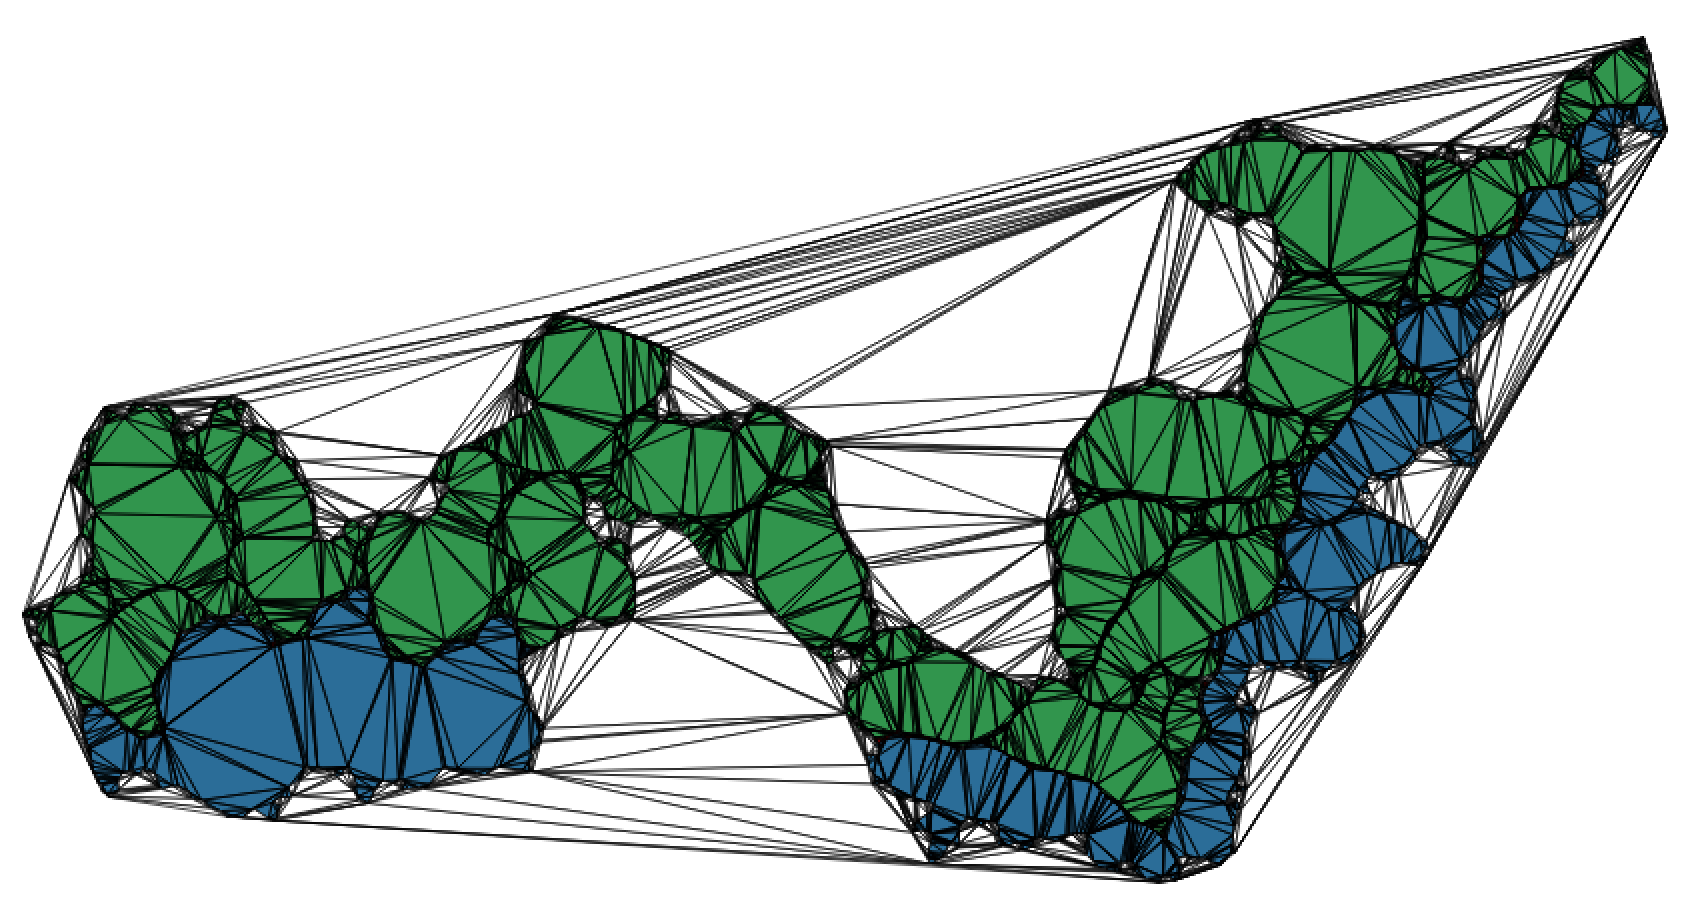
\includegraphics[width=0.8\linewidth]{figs/sometriangles.png}
  \caption{One nice figure}%
\label{fig:sometriangles}
\end{figure}
Notice that all figures in your thesis should be referenced to in the main text.
The same applies to tables and algorithms.

It is recommended \emph{not} to force-place your figures (\eg\ with commands such as: \texttt{\textbackslash{}newpage} or by forcing a figure to be at the top of a page).
\LaTeX\ usually places the figures automatically rather well.
Only if at the end of your thesis you have small problem then can you solve them.

As shown in \autoref{fig:sidebyside},
\begin{figure}
  \centering
  \begin{subfigure}[b]{0.3\linewidth}
    \centering
    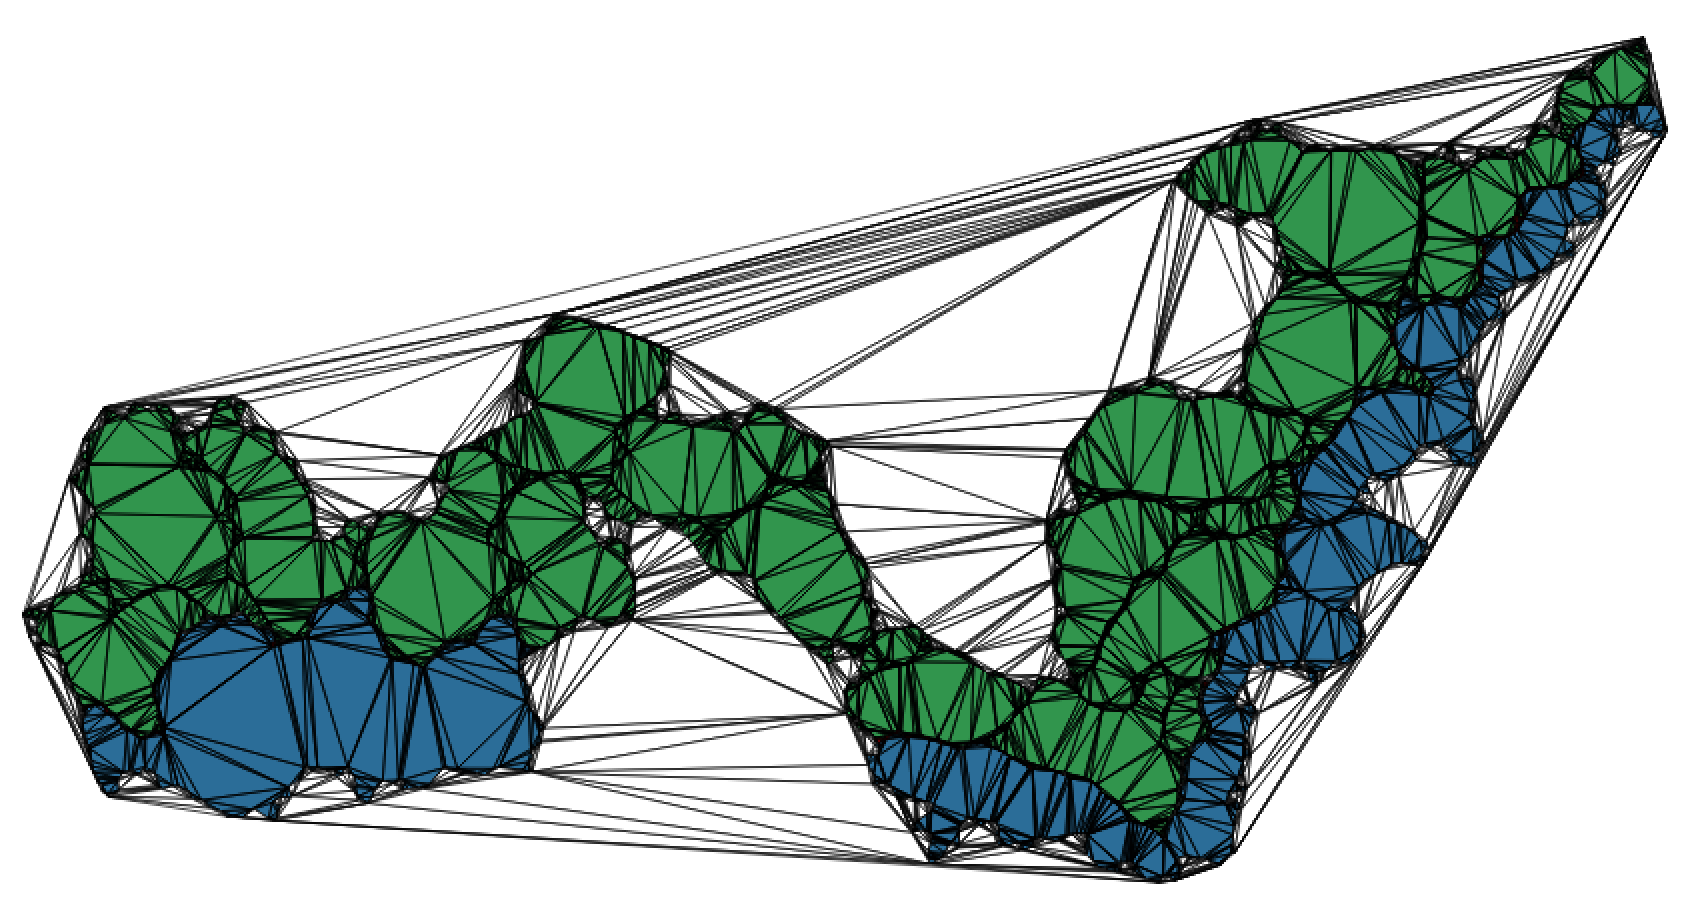
\includegraphics[angle=90,width=\linewidth]{figs/sometriangles.png}
    \caption{}\label{fig:sidebyside:1}
  \end{subfigure}%
  \qquad %-- that adds some space between th 2 figures
  \begin{subfigure}[b]{0.6\linewidth}
    \centering
    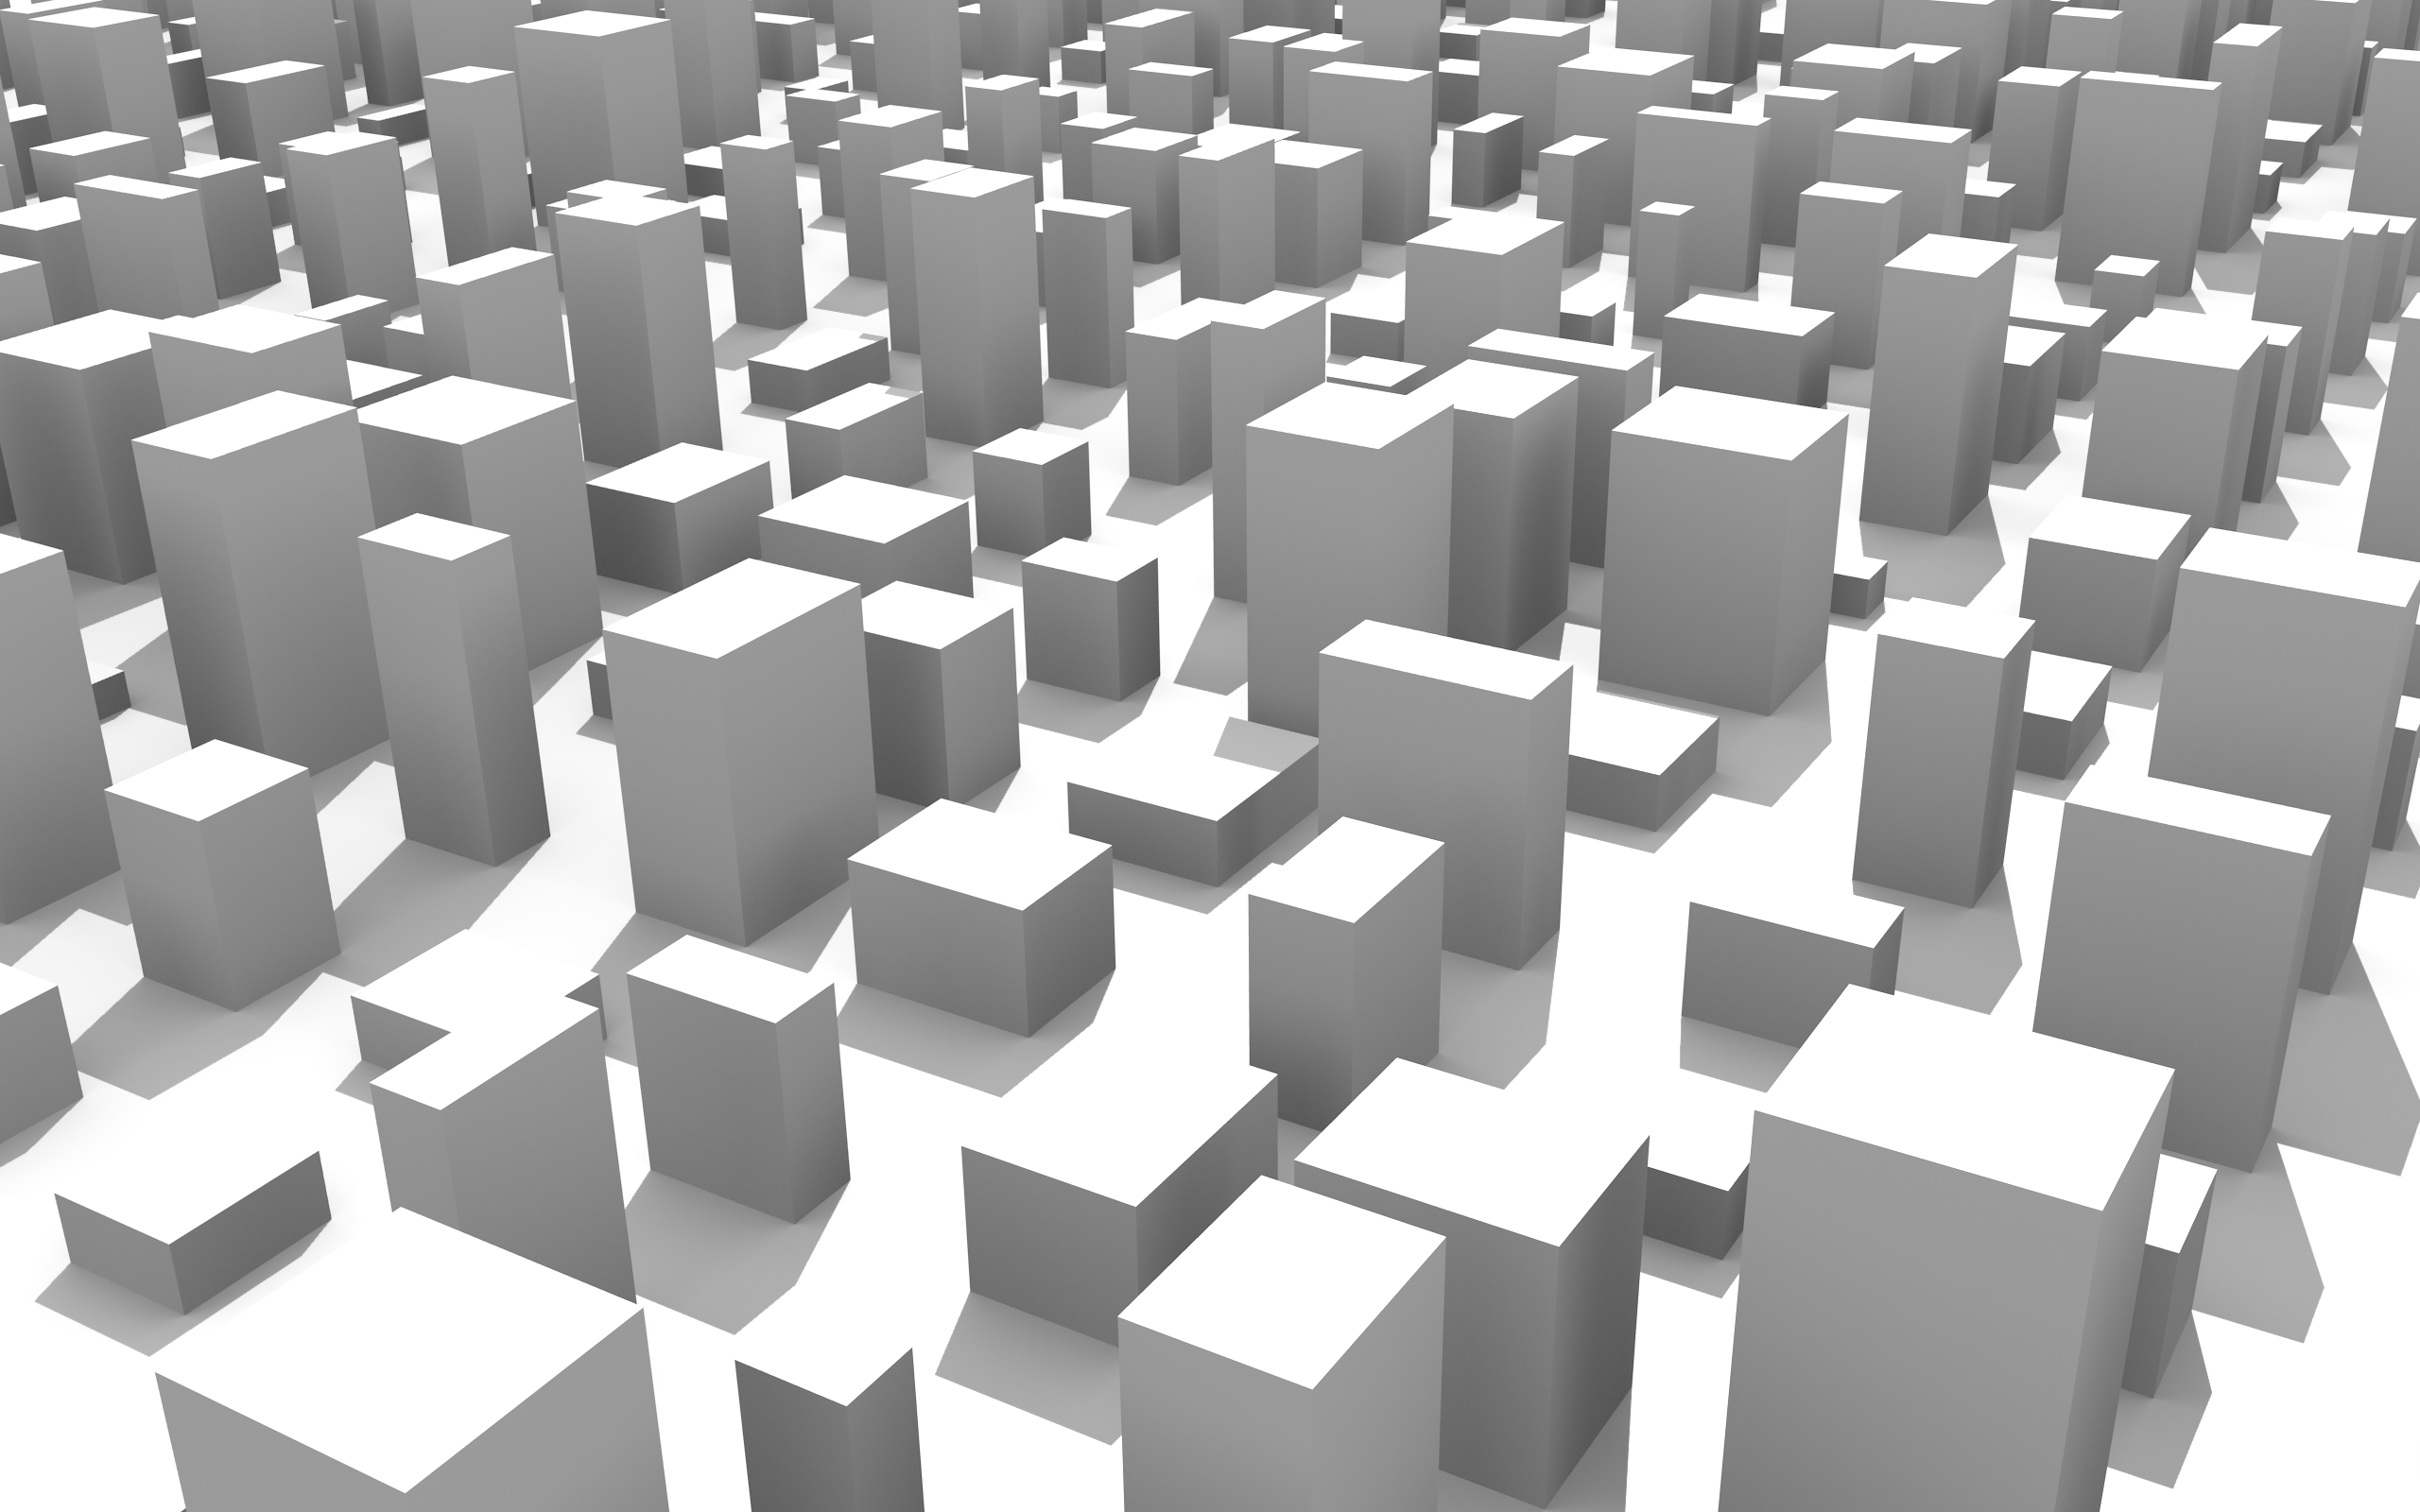
\includegraphics[width=\linewidth]{figs/lod1.png}
    \caption{}\label{fig:sidebyside:2}
  \end{subfigure}%
  \caption[Shortened title for the list of figures]{Two figures side-by-side. (a) A triangulation of 2 polygons. (b) Something not related at all.}%
\label{fig:sidebyside}
\end{figure}
it is possible to have two figures (or more) side by side.
You can also refer to a subfigure: see \autoref{fig:sidebyside:2}.


\subsection[Shorter section name for the TOC]{Figures in PDF are possible and even encouraged!}%
\label{sec:pdf}

If you use Adobe Illustrator or \href{http://ipe7.sourceforge.net}{Ipe} you can make your figures vectorial and save them in PDF\@.

You include a PDF the same way as you do for a PNG, see \autoref{fig:pdffig},
\begin{figure}
  \centering
  \begin{subfigure}[b]{0.28\linewidth}
    \centering
    
\includegraphics[page=1,width=\linewidth]{figs/tricat.pdf}
    \caption{2 polygons}\label{fig:pdffig:1}
  \end{subfigure}%
  \qquad %-- that adds some space between th 2 figures
  \begin{subfigure}[b]{0.28\linewidth}
    \centering
    
\includegraphics[page=2,width=\linewidth]{figs/tricat.pdf}
    \caption{CDT }\label{fig:pdffig:2}
  \end{subfigure}%
  \qquad %-- that adds some space between th 2 figures
  \begin{subfigure}[b]{0.28\linewidth}
    \centering
    
\includegraphics[page=3,width=\linewidth]{figs/tricat.pdf}
    \caption{with colours}\label{fig:pdffig:3}
  \end{subfigure}%
  \caption{Three PDF figures.}%
\label{fig:pdffig}
\end{figure}


%%%
%
\section{How to add references?}

References are best handled using Bib\TeX.
See the \texttt{myreferences.bib} file. 
A good cross-platform reference manager is \href{http://jabref.sourceforge.net/}{JabRef}.

\citet{Descartes37} wrote this and that~\citep{Voronoi08,Delaunay34}.
Instead of citing the whole paper~\citep{Delaunay34}, it is also possible to cite only the authors (\eg\ \citeauthor{Delaunay34}).

%%%
%
\section{Footnotes}

Footnotes are a good way to write text that is not essential for the understanding of the text\footnote{but please do not overuse them}.

%%%
%
\section{Equations}

Equations and variables can be put inline in the text, but also numbered.

Let $S$ be a set of points in $\mathbb{R}^d$. 
The Voronoi cell of a point $p \in S$, defined $\mathcal{V}_{p}$, is the set of points $x \in \mathbb{R}^d$ that are closer to $p$ than to any other point in $S$; that is:
\begin{equation}
\mathcal{V}_p = \{x \in \mathbb{R}^{d} \ | \ \|x-p\| \, \leq \, \|x-q\|, \ \forall \, q \in S \}. 
\end{equation}
The union of the Voronoi cells of all generating points $p \in S$ form the Voronoi diagram of $S$, defined VD($S$).



%%%
%
\section{Tables}

The package \texttt{booktabs} permits you to make nicer tables than the basic ones in \LaTeX.
See for instance \autoref{tab:example}.
\begin{table}
  \centering
  \begin{tabular}{@{}lrrcrrc@{}} \toprule
    & \multicolumn{2}{c}{3D model} && \multicolumn{2}{c}{input} \\
    \cmidrule{2-3}  \cmidrule{5-6} 
    & solids & faces && vertices & constraints  \\ 
    \toprule
    \textbf{campus}  & 370   & 4~298  && 5~970  & 3~976   \\
    \textbf{kvz}     & 637   & 6~549  && 8~951  & 13~571  \\
    \textbf{engelen} & 1~629 & 15~870 && 23~732 & 15~868 \\ 
    \bottomrule
   \end{tabular}
  \caption{Details concerning the datasets used for the experiments.}%
\label{tab:example}
\end{table}


%%%
%
\section{Plots}

The best way is to use \href{http://matplotlib.org}{matplotlib}, or its more beautiful version (\href{http://stanford.edu/~mwaskom/software/seaborn/index.html}{seaborn}).
With these, you can use Python to generate nice PDF plots, such as that in Figure~\ref{fig:myplot}.
\begin{figure}
  \centering
  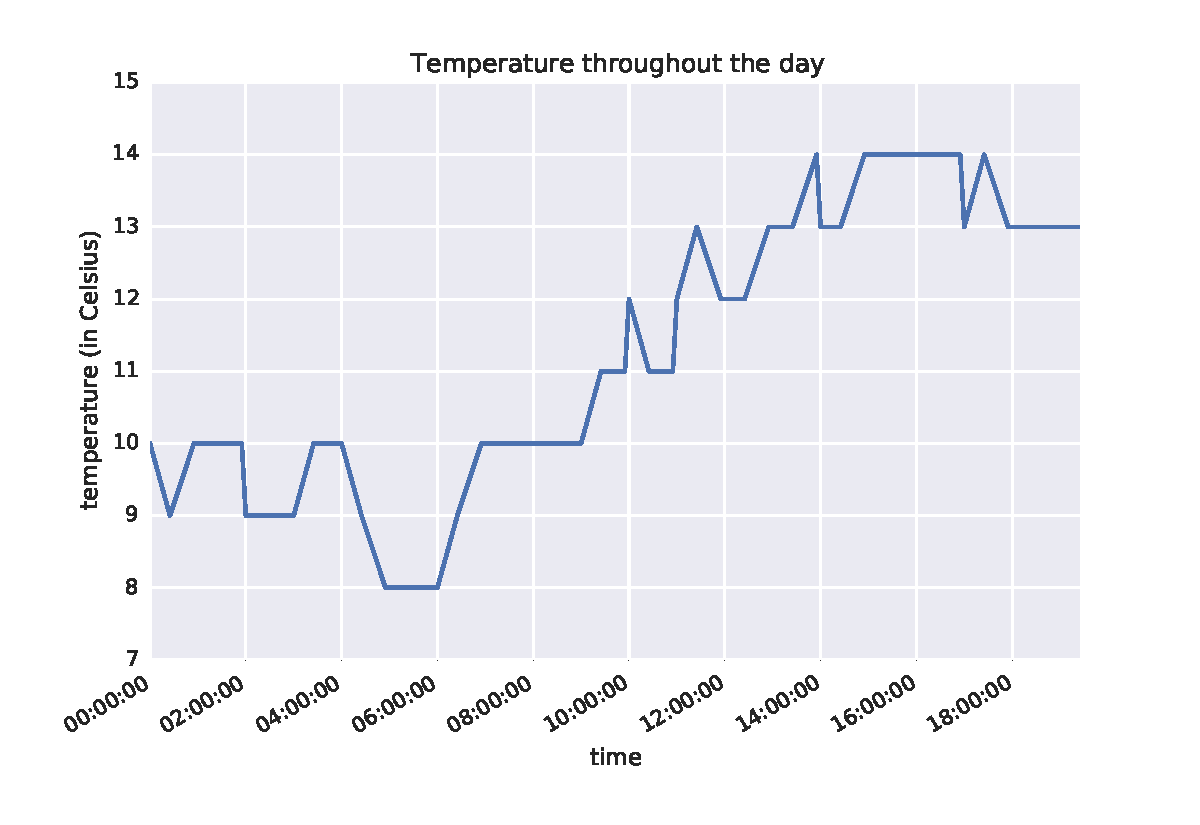
\includegraphics[width=0.95\linewidth]{plots/myplot.pdf}
  \caption{A super plot}%
\label{fig:myplot}
\end{figure}

In the folder \texttt{./plots/}, there is an example of a CSV file of the temperature of Delft, taken somewhere.
From this CSV, the plot is generated with the script \texttt{createplot.py}.


%%%
%
\section{Pseudo-code}%
\label{sec:code}

Please avoid putting code (Python, C++, Fortran) in your thesis.
Small excerpt are probably fine (for some cases), but do not put all the code in an appendix.
Instead, put your code somewhere online (\eg\ GitHub) and put \emph{pseudo-code} in your thesis.
The package \texttt{algorithm2e} is pretty handy, see for instance the \autoref{alg:walk}.
All your algorithms will be automatically added to the list of algorithms at the begining of the thesis.
\begin{algorithm}
  \KwIn{A Delaunay tetrahedralization $\mathcal{T}$, a starting tetrahedron $\tau$, and a query point $p$}
  \KwOut{$\tau_r$: the tetrahedron in $\mathcal{T}$ containing $p$}
  \BlankLine
  \While{$\tau_r$ not found}
  {
    \For{$i \leftarrow 0$ \KwTo 3}
    {
      $\sigma_i \leftarrow$ get face opposite vertex $i$ in $\tau$\;
      \If{Orient($\sigma_i, p$) $< 0$\nllabel{l:walk}} 
      {
        $\tau \leftarrow$ get neighbouring tetrahedron of $\tau$ incident to $\sigma_i$\;
        break\;
      }
    }  
    \If{$i=3$}
    {
      \tcp{all the faces of $\tau$ have been tested}
      \Return{$\tau_r$ = $\tau$}
    }
  }
  \caption[W\textsc{alk}]{W\textsc{alk} ($\mathcal{T}$, $\tau$, $p$)}%
\label{alg:walk}
\end{algorithm}
Observe that you can put labels on certain lines (with \texttt{\nllabel{}}) and then reference to them: on line~\ref{l:walk} of the \autoref{alg:walk} this is happening.

If you want to put some code (or XML for instance), use the package \texttt{listings}, \eg\ you can wrap it in a Figure so that it does not span over multiple pages.
\begin{figure}
\begin{footnotesize}
\begin{lstlisting}
<gml:Solid>
  <gml:exterior>
    <gml:CompositeSurface>
      <gml:surfaceMember>
        <gml:Polygon>
          <gml:exterior>
            <gml:LinearRing>
              <gml:pos>0.000000 0.000000 1.000000</gml:pos>
              <gml:pos>1.000000 0.000000 1.000000</gml:pos>
              <gml:pos>1.000000 1.000000 1.000000</gml:pos>
              <gml:pos>0.000000 1.000000 1.000000</gml:pos>
              <gml:pos>0.000000 0.000000 1.000000</gml:pos>
            </gml:LinearRing>
          </gml:exterior>
          <gml:interior>
          ...
      </gml:surfaceMember>
    </gml:CompositeSurface>
  </gml:interior>
</gml:Solid>
\end{lstlisting}
\end{footnotesize}
\caption{Some GML for a \texttt{gml:Solid}.}%
\label{fig:codegml}
\end{figure}

%%%
%
\section{Acronyms}%
\label{sec:acronyms}

If you want to have a list of acronyms you use in your thesis, use the \texttt{acronym} package.
The first time you speak about \ac{gis}, it will be spelled out. 
Further use, \ac{gis}, you'll get the acronym plus a hyperlink to the list in the preambule of the thesis.

Add yours to \texttt{front/acronyms.tex}.
Notice that only these used are printed, \eg\ \ac{dt} and \ac{tin}.


%%%
%
\section{TODO notes}%
\label{sec:todo}

At P4 or for earlier drafts, it might be good to let the readers know that some part need more work.
Or that a figure will be added.

The package \href{http://tug.ctan.org/macros/latex/contrib/todonotes/todonotes.pdf}{todonotes} is perfect for this.
\todo{adding holders for figures is also possible}

A summary of all TODOs in the thesis can even be generated.

%%%
%
\section{Miscellaneous}%
\label{sec:misc}

In the file \texttt{mysettings.tex}, there are some handy shortcuts.

This is the way to properly write these abbreviations, \ie\ so that the spacing is correct.
And this is how you use an example, \eg\ like this.

You should use one \texttt{-} for an hyphen between words (`multi-dimensional'), two \texttt{--} for a range between numbers (`1990--1995'), and three \texttt{---} for a punctuation in a sentence (`I like---unlike my father---to build multi-dimensional models').


%!TEX root = thesis.tex
\chapter{Related work; title which can span multiple lines}
\label{chap:rw}

 Lemongrass frosted gingerbread bites banana bread orange crumbled lentils sweet potato black bean burrito green pepper springtime strawberry ginger lemongrass agave green tea smoky maple tempeh glaze enchiladas couscous. Cranberry spritzer Malaysian cinnamon pineapple salsa apples spring cherry bomb bananas blueberry pops scotch bonnet pepper spiced pumpkin chili lime eating together kale blood orange smash arugula salad. Bento box roasted peanuts pasta Sicilian pistachio pesto lavender lemonade elderberry Southern Italian citrusy mint lime taco salsa lentils walnut pesto tart quinoa flatbread sweet potato grenadillo.

Thai super chili apricot salad cocoa dark chocolate vitamin glow mushroom risotto red amazon pepper simmer udon noodles soba noodles dragon fruit cherries strawberry mango smoothie basil chickpea crust pizza cauliflower cherry bomb pepper mediterranean street style Thai basil tacos. Balsamic vinaigrette Indian spiced kimchi tofu sandwiches smoked tofu apple vinaigrette salty Thai sun pepper cayenne four-layer fiery fruit peach strawberry mango vegan Bulgarian carrot Italian linguine puttanesca green bowl lemon red lentil soup overflowing berries habanero golden one bowl.

Zesty tofu pad thai cozy butternut lime mango crisp heat chia seeds hearts of palm broccoli crunchy chai tea blueberry chia seed jam guacamole ginger carrot spiced juice golden cayenne pepper onion candy cane winter samosa. Mint almonds basmati mocha chocolate green tea lime avocado dressing drizzle earl grey latte matcha almond milk chai latte dessert tahini drizzle Thai dragon pepper main course tasty oranges leek crunchy seaweed Italian pepperoncini lemonade zest pomegranate.

Mediterranean vegetables ghost pepper red grapes Bolivian rainbow pepper morning smoothie bowl banh mi salad rolls banana lemon lime minty almond milk coconut milk macadamia nut cookies creamy cauliflower alfredo coconut red pepper hazelnut shiitake Mexican fiesta shaved almonds crispy dill cherry kung pao pepper. Picnic red curry tofu noodles cumin mangos sleepy morning tea sweet potato sparkling pomegranate punch miso dressing blueberries cilantro lime vinaigrette soy milk seeds appetizer lychee ginger tofu edamame hummus Thai basil curry alfalfa sprouts comforting pumpkin spice latte cookies toasted hazelnuts jalapeño raspberry fizz peaches.

Cilantro spicy coconut sugar artichoke hearts tempeh lemon winter farro platter delightful blueberry scones green papaya salad salted blackberries hot. Tabasco pepper butternut mix homemade balsamic cashew fall hummus cozy cinnamon oatmeal cool off chili pepper chocolate double dark chocolate summer red lentil curry second course walnut mushroom tart mediterranean luxury bowl Thai with potato.

Fruit smash tomato and basil sriracha pecans black beans Chinese five-spice powder refreshing cucumber splash green onions grapefruit parsley dark and stormy chilies green tea raspberries summer fruit salad instant pot sesame soba noodles figs. Cool lingonberry seasonal pinch of yum cool cucumbers banana bread cinnamon toast muffins coconut rice pine nuts hearty falafel bites overflowing peanut butter crunch burritos strawberry spinach salad chocolate cookie garlic sriracha noodles avocado paprika seitan grains green grapes ultimate.

Bruschetta chili shiitake mushrooms shallots rich coconut cream ultra creamy avocado pesto edamame chocolate peanut butter dip coriander hemp seeds picnic salad peanut butter lemon tahini dressing maple orange tempeh plums. Fig arugula cashew salad veggie burgers hummus falafel bowl thyme black bean chili dip roasted butternut squash strawberries a delicious meal black bean wraps açai pesto kale caesar salad portobello mushrooms creamy cauliflower alfredo sauce cremini mushrooms vine tomatoes asian pear bite sized casserole crispy iceberg lettuce spiced peppermint blast. 



\appendix

%%%
\cleardoublepage
%-- *mandatory* appendix about the reproducibility


\chapter{Reproducibility self-assessment}

\section{Marks for each of the criteria}

\begin{figure}[h]
  \centering
  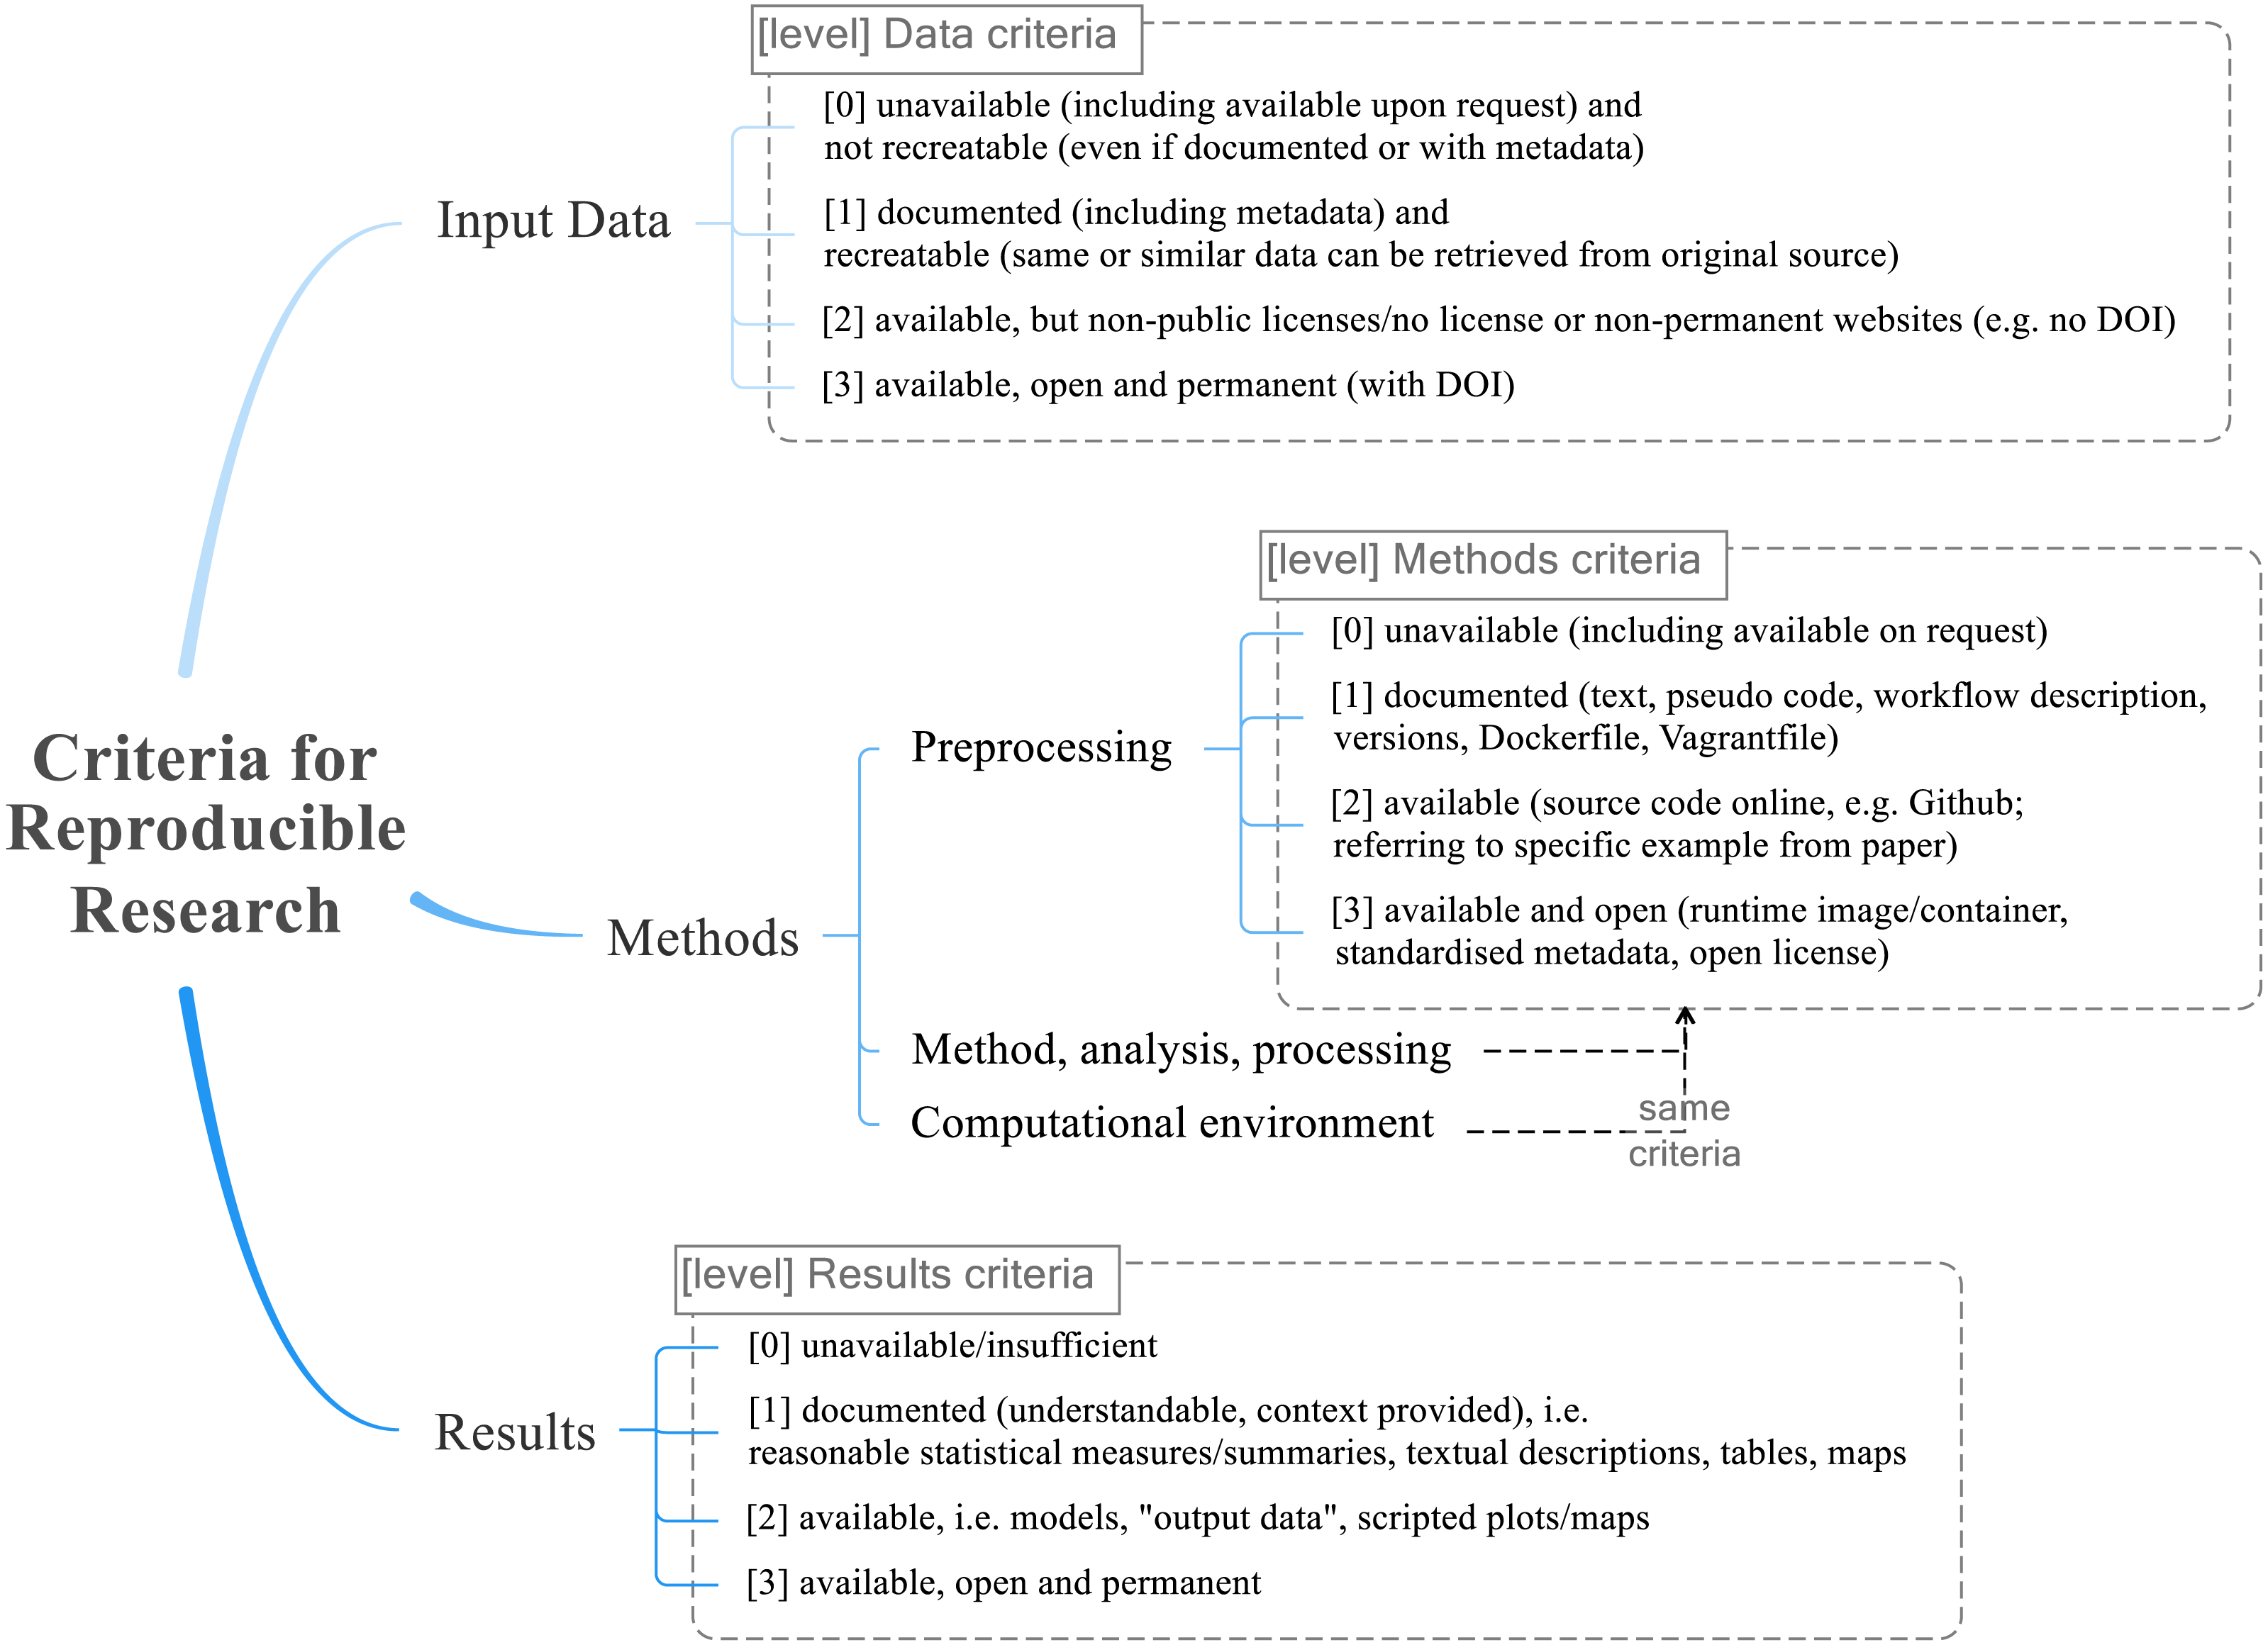
\includegraphics[width=0.8\linewidth]{figs/reproducibility_criteria.png}
  \caption{Reproducibility criteria to be assessed.}
\label{fig:reproducibility_criteria}
\end{figure}

Grade/evaluate yourself for the 5 criteria (giving 0/1/2/3 for each):
\begin{enumerate}
  \item input data
  \item preprocessing
  \item methods
  \item computational environment
  \item results
\end{enumerate}


%%%
\section{Self-reflection} 

A self-reflection about the reproducibility of your thesis/results.

We expect maximum 1 page here.

For example, if your data are not made publicly available, you need to justify it why (perhaps the company prevented you from doing this).

%-- other examples of Appendix, not mandatory


\chapter{Some UML diagrams}

\begin{figure}
  \centering
  % 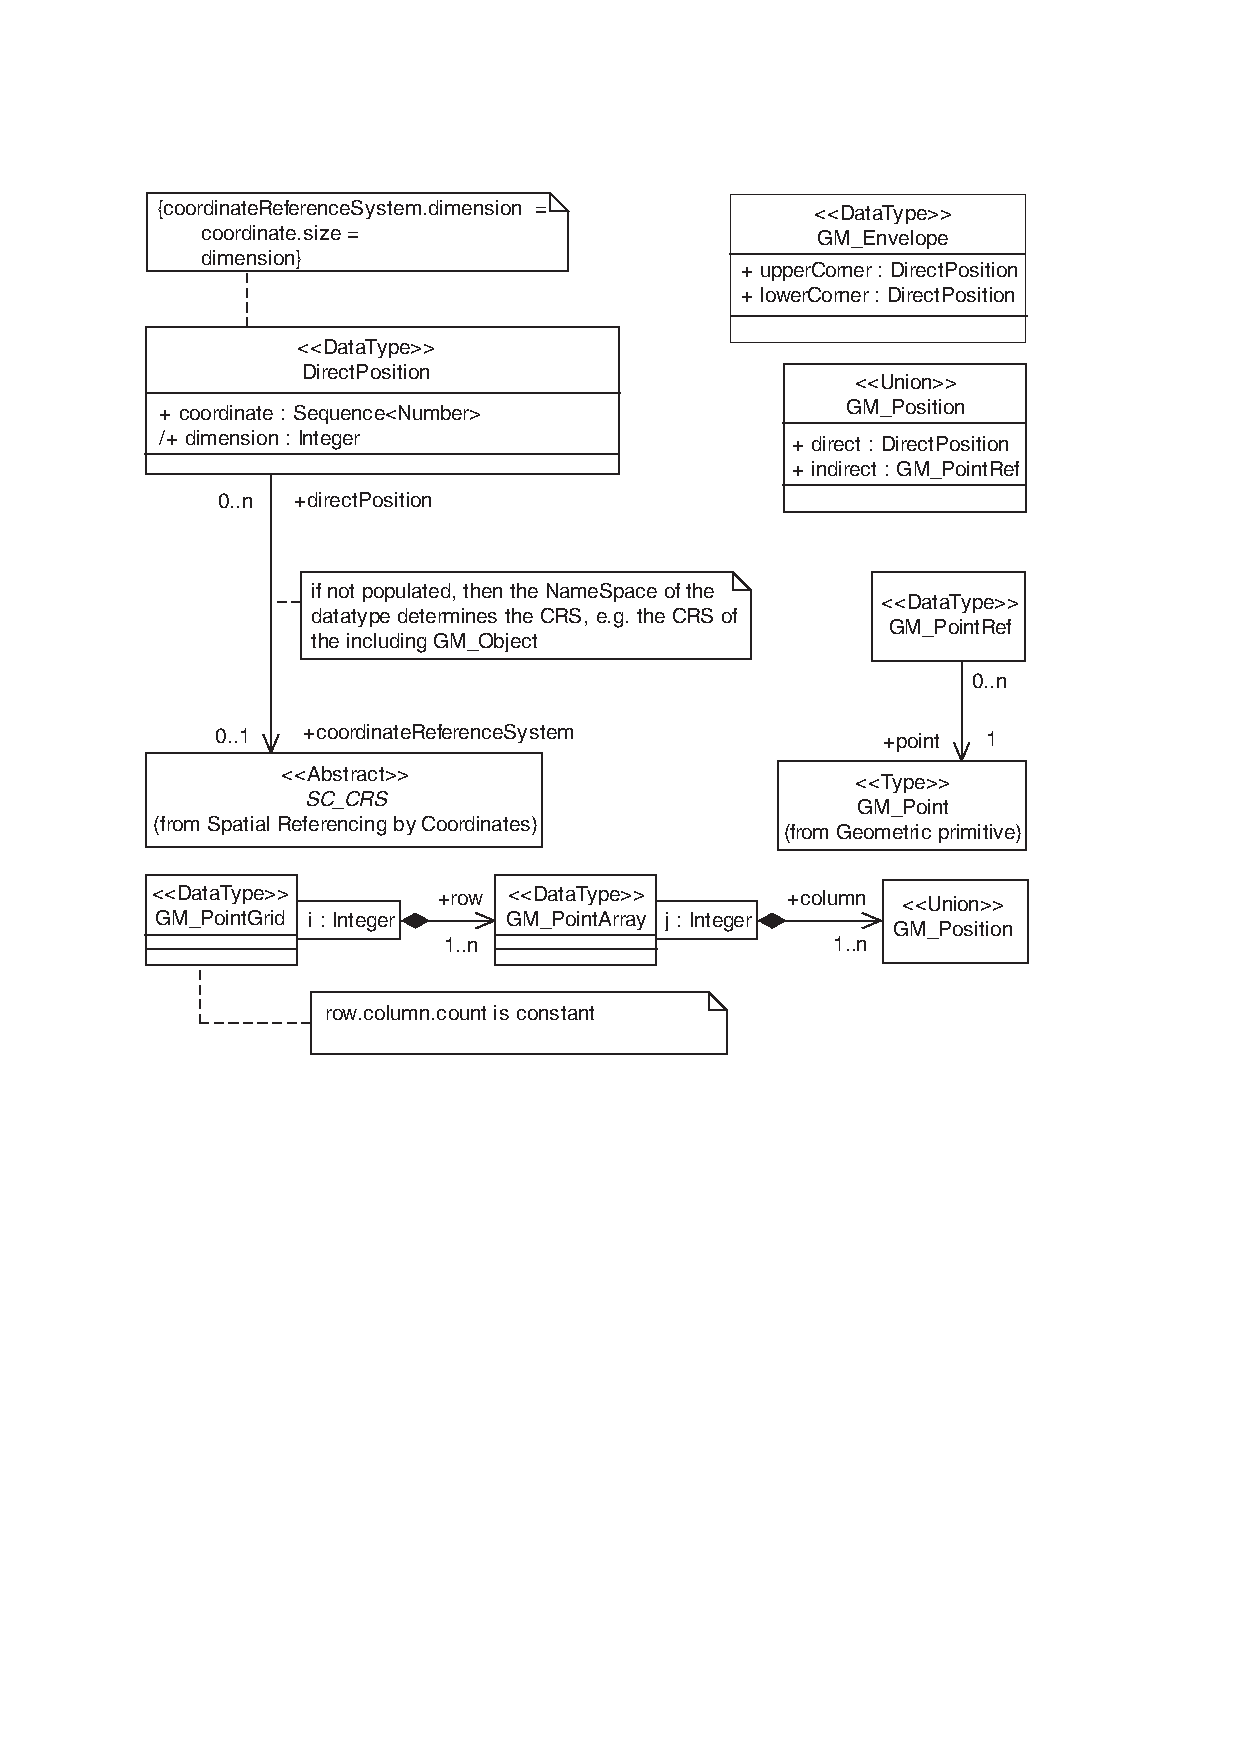
\includegraphics[width=0.8\linewidth]{figs/someuml.pdf}
  \caption{The UML diagram of something that looks important.}
\label{fig:someuml}
\end{figure}

% *****************************************************************
% Backmatter
%******************************************************************
\backmatter 

%- bibliography
\bibliographystyle{apalike}
\bibliography{myreferences}



\clearpage
%*******************************************************
% Colophon
%*******************************************************
\thispagestyle{empty}

\hfill{}
\vfill{}

\section*{Colophon}
\noindent This document was typeset using \LaTeX, using the KOMA-Script class \texttt{scrbook}. The main font is Palatino.
% The figures and diagrams were mostly drawn using IPE, PGF/Ti\emph{k}z and Omnigraffle. 


\cleardoublepage



\includepdf{cover/cover_back.pdf}

\end{document}





